% ============================================================================
% Shared main-body figure definitions.
% Figure assets are included under figures/.
% ============================================================================

\begin{figure*}[!t]
  \centering
  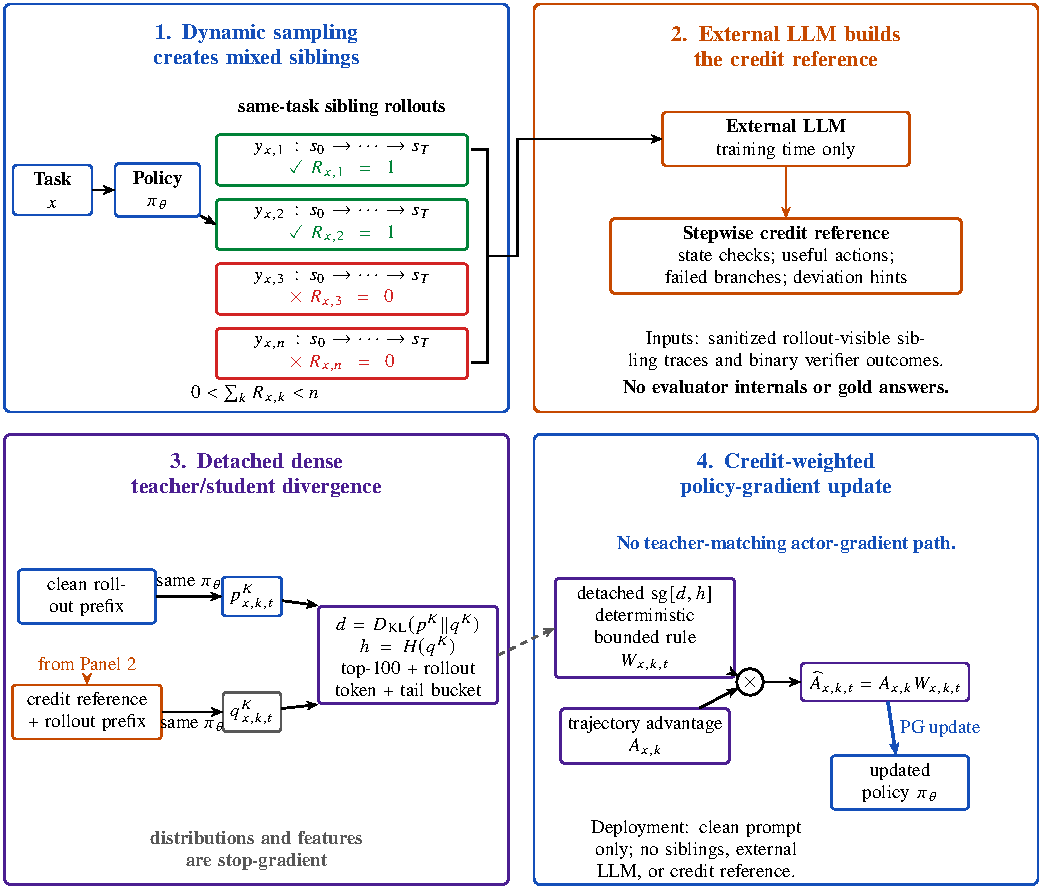
\includegraphics[width=\textwidth]{f3_method_schematic.pdf}
  \caption{\method overview. Dynamic sampling creates mixed sibling rollouts;
    an external LLM summarizes their contrast into a training-only stepwise
    credit reference; detached dense teacher/student divergence produces
    credit features; and bounded credit weights reweight the policy-gradient
    advantage. The inference-time student receives only the clean task prompt.
    The schematic shows only SGCD-specific paths: the detached divergence
    pathway contributes no teacher-matching actor gradient. The reference-KL
    used by the Vanilla GRPO comparators is outside this SGCD schematic; SGCD
    uses no reference-KL.}
  \label{fig:method}
\end{figure*}
